\documentclass[10pt,a4paper]{article}
\usepackage{lmodern}

\usepackage{amssymb,amsmath}
\usepackage{ifxetex,ifluatex}
\usepackage{fixltx2e} % provides \textsubscript
\ifnum 0\ifxetex 1\fi\ifluatex 1\fi=0 % if pdftex
\usepackage[T1]{fontenc}
\usepackage[utf8]{inputenc}
\else % if luatex or xelatex
\ifxetex
\usepackage{mathspec}
\usepackage{xltxtra,xunicode}
\else
\usepackage{fontspec}
\fi
\defaultfontfeatures{Mapping=tex-text,Scale=MatchLowercase}
\newcommand{\euro}{€}
\fi
% use upquote if available, for straight quotes in verbatim environments
\IfFileExists{upquote.sty}{\usepackage{upquote}}{}
% use microtype if available
\IfFileExists{microtype.sty}{%
	\usepackage{microtype}
	\UseMicrotypeSet[protrusion]{basicmath} % disable protrusion for tt fonts
}{}
\usepackage[lmargin=2.5cm,rmargin=2.5cm,tmargin=2.5cm,bmargin=2.5cm]{geometry}

% Figure Placement:
\usepackage{float}
\let\origfigure\figure
\let\endorigfigure\endfigure
\renewenvironment{figure}[1][2] {
	\expandafter\origfigure\expandafter[H]
} {
	\endorigfigure
}

%% citation setup

\usepackage{csquotes}

\usepackage[backend=biber, maxbibnames = 99, style = apa]{biblatex}
\setlength\bibitemsep{1.5\itemsep}
\bibliography{references\_tidy.bib}
\usepackage{graphicx}
\makeatletter
\def\maxwidth{\ifdim\Gin@nat@width>\linewidth\linewidth\else\Gin@nat@width\fi}
\def\maxheight{\ifdim\Gin@nat@height>\textheight\textheight\else\Gin@nat@height\fi}
\makeatother
% Scale images if necessary, so that they will not overflow the page
% margins by default, and it is still possible to overwrite the defaults
% using explicit options in \includegraphics[width, height, ...]{}
\setkeys{Gin}{width=\maxwidth,height=\maxheight,keepaspectratio}
\ifxetex
\usepackage[setpagesize=false, % page size defined by xetex
unicode=false, % unicode breaks when used with xetex
xetex]{hyperref}
\else
\usepackage[unicode=true]{hyperref}
\fi
\hypersetup{breaklinks=true,
	bookmarks=true,
	pdfauthor={Ignacio Moreira Lara, Stefan Linner, Konstantin Lehmann},
	pdftitle={tidyMC},
	colorlinks=true,
	citecolor=blue,
	urlcolor=blue,
	linkcolor=magenta,
	pdfborder={0 0 0}}
\urlstyle{same}  % don't use monospace font for urls
\setlength{\parindent}{0pt}
\setlength{\parskip}{6pt plus 2pt minus 1pt}
\setlength{\emergencystretch}{3em}  % prevent overfull lines
\setcounter{secnumdepth}{0}

%%% Use protect on footnotes to avoid problems with footnotes in titles
\let\rmarkdownfootnote\footnote%
\def\footnote{\protect\rmarkdownfootnote}

%%% Change title format to be more compact
\usepackage{titling}

% Create subtitle command for use in maketitle
\newcommand{\subtitle}[1]{
	\posttitle{
		\begin{center}\large#1\end{center}
	}
}

\setlength{\droptitle}{-2em}
\title{tidyMC}
\pretitle{\vspace{\droptitle}\centering\huge}
\posttitle{\par}
\subtitle{An easy-to-use package for Monte-Carlo Simulations}
\author{Ignacio Moreira Lara, Stefan Linner, Konstantin Lehmann}
\preauthor{\centering\large\emph}
\postauthor{\par}
\predate{\centering\large\emph}
\postdate{\par}
\date{2022-08-29}

\usepackage{lmodern}
\usepackage{mathtools}
\usepackage{amsmath}
\usepackage{amsfonts}
\usepackage{soul}
\usepackage{booktabs}
\usepackage{longtable}
\usepackage{array}
\usepackage{multirow}
\usepackage{wrapfig}
\usepackage{float}
\usepackage{colortbl}
\usepackage{pdflscape}
\usepackage{tabu}
\usepackage{threeparttable}
\usepackage{threeparttablex}
\usepackage[normalem]{ulem}
\usepackage{makecell}
\usepackage{xcolor}

% Multicols for the Title page
\usepackage{multicol}

\usepackage{longtable}


%% linespread settings

\usepackage{setspace}

\onehalfspacing

% Language Setup

\usepackage{ifthen}
\usepackage{iflang}
\usepackage[super]{nth}

\ifthenelse{\equal{english}{german}}{
	\usepackage[ngerman]{babel}
}{
	\usepackage[english]{babel}
}

\begin{document}
	
	\newgeometry{left=2.5cm,right=1cm,bottom=2cm,top=2cm}
	
	\begin{titlepage}
		\noindent\begin{minipage}{0.6\textwidth}
			\IfLanguageName{english}{University of Duisburg-Essen}{Universität Duisburg-Essen}\\
			\IfLanguageName{english}{Faculty of Business Administration and Economics}{Fakultät für Wirtschaftswissensschaften}\\
			\IfLanguageName{english}{Chair of Econometrics}{Lehrstuhl für Ökonometrie}\\
		\end{minipage}
		\begin{minipage}{0.4\textwidth}
			\begin{flushright}
				\vspace{-0.5cm}
				\IfLanguageName{english}{\includegraphics*[width=5cm]{Includes/duelogo_en.png}}{\includegraphics*[width=5cm]{Includes/duelogo_de.png}}
			\end{flushright}
		\end{minipage}
		\\
		\vspace{1.5cm}
		\begin{center}
			\huge{tidyMC}\\
			\vspace{.25cm}
			\Large{An easy-to-use package for Monte-Carlo Simulations}\\
			\vspace{0.5cm}
			\large{Report}\\
			\vspace{1cm}
			\large{
				\IfLanguageName{english}{Submitted to the Faculty of \\ Business Administration and Economics \\at the \\University of Duisburg-Essen}{Vorgelegt der \\Fakultät für Wirtschaftswissenschaften der \\ Universität Duisburg-Essen}\\}
			\vspace{0.75cm}
			\large{\IfLanguageName{english}{from:}{von:}}\\
			\vspace{0.5cm}
			Ignacio Moreira Lara, Stefan Linner, Konstantin Lehmann\\
		\end{center}
		\vfill
		\hrulefill
		
		\noindent\begin{minipage}[t]{0.3\textwidth}
			\IfLanguageName{english}{First Reviewer:}{Erstgutachter:}
		\end{minipage}
		\begin{minipage}[t]{0.7\textwidth}
			\hspace{1cm}Jens Klenke 
		\end{minipage}
	
			\noindent\begin{minipage}[t]{0.3\textwidth}
			\IfLanguageName{english}{Second Reviewer:}{Zweitertgutachter:}
		\end{minipage}
		\begin{minipage}[t]{0.7\textwidth}
			\hspace{1cm}Martin C. Arnold 
		\end{minipage}
	
		\noindent\begin{minipage}[t]{0.3\textwidth}
			\IfLanguageName{english}{Deadline:}{Abgabefrist:}
		\end{minipage}
		\begin{minipage}[t]{0.7\textwidth}
			\hspace{1cm}06.09.2022
		\end{minipage}
	\vfill
		\hrulefill
		
		\begin{multicols}{4}
			
			Name:
			
			Matriculation No.:
			
			E-Mail:
			
			Study Path:
			
			Semester:
			
			Graduation (est.):
			
			\columnbreak
			
			Ignacio Moreira
			
			230658
			
			ignacio.moreira-lara@tu-dortmund.de
			
			M.Sc. Econometrics
			
			\nth{4}
			
			Summer Term 2022
			
			\columnbreak
			
			Stefan Linner
			
			233565
			
			stefan.linner@tu-dortmund.de
			
			M.Sc. Econometrics
			
			\nth{2}
			
			Summer Term 2022
			
			\columnbreak
			
			Konstantin Lehmann
			
			229994
			
			konstantin.lehmann@tu-dortmund.de
			
			M.Sc. Econometrics
			
			\nth{4}
			
			Summer Term 2022
			
		\end{multicols}
		
	\end{titlepage}
	
	% Ends the declared geometry for the titlepage
	\restoregeometry
	
		
		
				\newpage
	\pagenumbering{arabic} 
	\hypertarget{introduction}{%
 \section{Introduction}\label{introduction}}

 Monte Carlo Simulations (henceforth MCS) are used to study the
 properties of econometrics inference techniques by simulation. They are
 almost always part of theoretical econometric research to study the
 performance of some inference technique. They supplement theoretical
 research most often in one of four ways. Firstly, they are often used
 to assess the performance of asymptotically valid techniques in smaller
 samples. Secondly, they are often used to assess how robust a technique
 is to violations of its theoretical assumptions. Thirdly, they allow to
 compare the performance of different techniques for a given data
 generating process (DGP). Fourthly, MCS allows to investigate the
 properties of inference techniques for which no analytical solution
 exists. Moreover, MCS itself can be used as a statistical inference
 technique itself. For example, Bootstrap Inference can be
 conceptualized as a special case of MCS. Beyond these examples, there
 are many more areas where MCS is used. However, independent of its
 use-case, easy and efficient implementation of MCS is currently only
 sparsely available.

 With our \texttt{tidyMC} package, we want to enable researchers to
 easily and efficiently include MCS in their research using the
 programming language R. For one, \texttt{`tidyMC`} allows to easily
 speed up MCS by providing efficient parallelization options over a
 pre-specified parameter grid. Because MCS involves repeated
 computation, using parallel workers allows for significant computation
 time reductions. For another, \texttt{`tidyMC`} returns an easy to work
 with output. The output allows to access the result of all simulations
 for every parameter combination in the parameter grid. Moreover,
 \texttt{`tidyMC`} provides functions to effectively communicate the
 results of the MCS. Using the output, the simulation results can then
 be easily visualized using the package's plot function. Because the
 function returns a ggplot object, researchers can customize the object
 to their liking. Additionally, the package provides a function that
 converts the results into publication-ready LaTex tables. The table is
 heavily customizable and thereby allows researchers to effectively
 communicate their results.

 This report is structured as follows. Section
 @ref(monte-carlo-simulation) gives an introduction to why and how Monte
 Carlo simulations work and provides a simple OLS example. Section
 @ref(package-principles) explains the coding practices we followed and
 gives a conceptual overview of how we implemented MCS in R. Section
 @ref(vignette) presents tidyMC's vignette. The vignette gives an
 easy-to-follow guide on how to implement MCS using the tidyMC package.
 Section @ref(comparison-to-other-monte-carlo-approaches-in-r) compares
 the performance of tidyMC to the performance of the MonteCarlo package
 and other potential MCS implementations. Section @ref(conclusion)
 concludes.

 \hypertarget{monte-carlo-simulation-mcs}{%
 \section{Monte Carlo Simulation
 \{MCS\}}\label{monte-carlo-simulation-mcs}}

 MCS allow analyzing the properties of classic econometric inference
 techniques. As a simulation-based technique, MCS applies a statistical
 procedure to many synthetically created samples. The repeated
 application of the procedure to a fully known DGP helps to investigate
 properties of statistical techniques in two situations. For one, it
 allows to scrutinize the properties of asymptotically consistent
 estimators in smaller samples. For another, it helps to analyze
 properties in situations which are analytically not solvable. In this
 section we want to give a brief overview how and in which circumstances
 work, mainly following.

 \hypertarget{pseudo-random-number-generation-and-the-data-generating-process}{%
 \subsection{Pseudo Random Number Generation and the Data Generating
 Process}\label{pseudo-random-number-generation-and-the-data-generating-process}}

 Using MCS on computers has the great advantage that, with the necessary
 information, the simulations results can be replicated everywhere. This
 is possible because, given seed and algorithm, the numbers created by a
 random number generator are completely reproducible. MCS generally
 starts with a synthetically created i.i.d. sample. Computers are,
 however, not able to generate truly random draws from different
 distributions. Instead the computer's draws from different
 distributions that are generated through pseudo-random draws from a
 uniform distribution. While we do not provide a detailed description of
 the different algorithms used, we explain the underlying intuition
 behind random number generation.

 Creating pseudo-random numbers from a probability distribution
 generally requires creating pseudo-random draws from a standard uniform
 distribution. Draws from a uniform distribution are created through the
 application of a certain algorithm, called random number generators
 (RNG), to a natural number, called the seed. The created values are
 pseudo-random because they are indistinguishable from truly random
 numbers but are fully determined by the combination of the algorithm
 and the seed. Combined knowledge of the algorithm and the seed allows
 exact replication of a series of pseudo-random numbers generated. The
 possibility to replicate the draws allows to exactly reproduce results
 that build on the pseudo-randomly generated number on different
 computers.

 The most common algorithm, as well as R's standard algorithm, used for
 the generation of pseudo-random draws from a standard uniform
 distribution, is the Mersenne-Twister algorithm. There are however more
 algorithms available. In R it is also possible to specify your own
 algorithm to create pseudo-random numbers. The purpose of the
 tidyMC-package is to additionally allow easy parallelization od the
 MCS. With parallel computing, special attention has to be payed to
 create disjoint and sufficiently long sets of draws from a uniform
 distribution. Our package builds on R-standard L'Ecuyer-CMRG RNG
 streams. The algorithm creates reproducible sets of \(U[0,1]\) numbers
 for each parallel worker, using an integer seed of length 7.
 Alternatively a seed of length 1 is accepted, which corresponds to a
 valid seed of length 7. Because the algorithm creates a subset of
 random numbers for each workers, the stream and hence the MCS results
 are only reproducible if the same number of parallel workers is used.
 Alternatively our function allows to supply user-generated lists of
 random variables.

 Generating pseudo-random numbers from more complex distributions uses
 the distribution's cumulative distribution function (CDF). It can be
 shown that every random variable \(X\) has a CDF \(F\) if
 \(X = F^{-1}(U)\), where U is a random variable uniformly distributed
 on \((0,1)\). Pseudo-random draws from different probability
 distributions are conceptually implemented by applying the inverse of
 CDF to pseudo-random numbers from the uniform distribution. Direct
 application of the inverse CDF is however often computationally
 time-consuming and requires that the inverse CDF is analytically
 available. To account for the two shortcomings different approaches
 have been developed for specific distributions, that also easily extend
 to random vectors. While they build on the idea to use the inverse of
 the CDF, their concrete design is out of the scope of this paper. A
 general overview can be found in the documentation of the respective
 R-functions.

 Complex multivariate distribution can then be simulated as functions of
 standard distributions. A typical example of that is a linear
 conditional expectation functions, the work horse model of
 econometrics. In the following example, we will showcase how MCS allows
 to simulate the correct distribution of the coefficients.

 \hypertarget{monte-carlo-distrbution-approximation}{%
 \subsection{Monte Carlo Distrbution
 Approximation}\label{monte-carlo-distrbution-approximation}}

 MCS is most commonly used to infer properties of the distribution of
 statistic in a fixed settting, i.e.~for a prespecified DGP. The
 simulation results hence hold only for the prespecified DGP. Because it
 additionally only approximates the distribution numerically, we need to
 control for the resulting approximation inaccuracies.

 In MCs we generally simulate the distribution of a statistic \(q_n\).
 The statistic can often be expressed as a function of a parameter
 vector \(\beta\), some deterministic variables \(D\) and some random
 variables \(v\), s.t. \(q_n = q_n(\theta,D,v,n)\). What a Monte Carlos
 simulation ultimately achieves is a numerical approximation of the true
 distribution of \(q_n\). In a simple i.id. setting an application of
 the CLT. Let \(q_n^R\) be the statistic generate by the \(R^th\) Monte
 Carlo Simulation. What we get is that as the histogram of all \(q_n^R\)
 becomes a unbiased and consistent estimator of \(q_n\). ADD THE FORMAL
 STUFF HERE. p.36! And add here discontciotn between histogram and We
 are hence able to control the precision of the approximation by setting
 the number of Monte Carlo estimates. Using the resulting distribution
 \(q_n^R\) we can then use different statistics such as mean and
 variance to summarize the result.

 \hypertarget{presenting-mcs-findngs}{%
 \subsubsection{Presenting MCS findngs}\label{presenting-mcs-findngs}}

 p.~122 add maybe here?

 \hypertarget{monte-carlo-example}{%
 \section{Monte Carlo example}\label{monte-carlo-example}}

 \hypertarget{ols-consistency}{%
 \subsection{OLS consistency}\label{ols-consistency}}

 To demonstrate how a MCS works, we provide an example using the
 estimation of a linear model using the ordinary least squares(OLS)
 estimator. Given a dependent variable \(y\) and a set of i.id.
 regressors \(X = \{x_1, x_2\}\) we consider the linear DGP
 \begin{equation}
     \label{eq_DGP}
     y = \beta_0 + \beta_1 x_1 + \beta_2 x_2 + \varepsilon,
 \end{equation}\\
 where \(\beta = \{\beta_0, \beta_1, \beta_2\}\) are the coefficients
 and \(\varepsilon\) is a normally distributed error term with variance
 \(\sigma^2\), i.e.~\(\varepsilon \sim \mathcal{N}(0,\sigma^2)\). The
 corresponding OLS estimators \(\hat{beta}\) and \(s^2\) for \(\beta\)
 and \(\sigma^2\) are \begin{align}
     \hat{\beta} = (XX)^{-1} XY,\\
     s^2 =   \frac{1}{n-k} \hat{\varepsilon}' \hat{\varepsilon},
 \end{align} where \(k = 2\) is the number of regressors and
 \(\hat{\varepsilon}\) is the vector of residuals. Both estimators are
 consistent and unbiased. Accordingly OLS should be able to correctly
 estimate the coefficients for every sample size, while the precision of
 the estimates should increase in the sample size.

 \noindent Using a MCS we can demonstrate the properties of the OLS
 estimator. Fixing the coefficients \(\beta = \{1, 4, 5\}\) and
 \(\sigma^2 = 3\), we generate different DGPs using different normal
 distributions to generate the dependent variables \(x_1\) and \(x_2\).
 Additionally, we generate \(\varepsilon\) from its respective
 distribution, and we estimate OLS on this sample. The number of
 observations we use is set to \(n = \{100, 200, 300\}\), which will be
 used to assess the convergence of the OLS estimators. We repeat the
 estimation 10000 times for each \(n\).

 We present the results in table \ref{tab:ols_table}, where the first
 column is related to the number of observations we use in the
 estimation. The last 4 columns show the results' mean over for each
 parameter combination up to an specific repetition number. In the first
 panel the mean over the estimated coefficients from the ten first
 repetitions is calculated; the subsequent panel shows the mean
 calculated using all Monte Carlo repetitions. The results demonstrate
 the performance of OLS estimation with increasing sample sizes. As
 expected figure \l\{(XX)\} and table \hl{(XX)} confirm that a bigger
 sample size leads to a more precise estimation of the underlying
 population values. Comparing both panels, we see that this behavior is
 just confirmed, as the estimated values do not differ and they become
 more precise.

 \begin{table}[H]

 \caption{\label{tab:ols_table}OLS consistency MC results}
 \centering
 \begin{tabular}[t]{ccccc}
 \toprule
 Number of observations & $\beta_0$ & $\beta_1$ & $\beta_2$ & $s^2$\\
 \midrule
 \addlinespace[0.3em]
 \multicolumn{5}{l}{\textbf{N = 10}}\\
 \hspace{1em}100 & 1.000 & 4.031 & 5.000 & 2.908\\
 \hspace{1em}200 & 0.944 & 4.005 & 5.010 & 2.860\\
 \hspace{1em}300 & 0.985 & 3.986 & 4.995 & 3.004\\
 \addlinespace[0.3em]
 \multicolumn{5}{l}{\textbf{N = 10000}}\\
 \hspace{1em}100 & 0.997 & 4.000 & 5.000 & 2.935\\
 \hspace{1em}200 & 1.000 & 4.000 & 5.000 & 2.969\\
 \hspace{1em}300 & 1.002 & 4.000 & 5.000 & 2.981\\
 \bottomrule
 \multicolumn{5}{l}{\rule{0pt}{1em}\textit{Note: }}\\
 \multicolumn{5}{l}{\rule{0pt}{1em}Total repetitions = 10000, total parameter combinations = 3}\\
 \end{tabular}
 \end{table}

 Similarly to show the convergence of the estimators in a graphical
 manner, we present histograms of the estimated coefficients for all
 values of \(n\). We present the densities for \(\hat{\beta_1}\) and
 \(s^2\) in figures \ref{fig:ols_b1} and \hl{(XX)}, and include the
 remaining plots in the Appendix. The pattern for both figures is clear,
 the increase in \(n\) reduces the variance of the estimator around the
 true value, thus the convergence of the OLS estimators is empirically
 visible.

 \begin{figure}
 \centering
 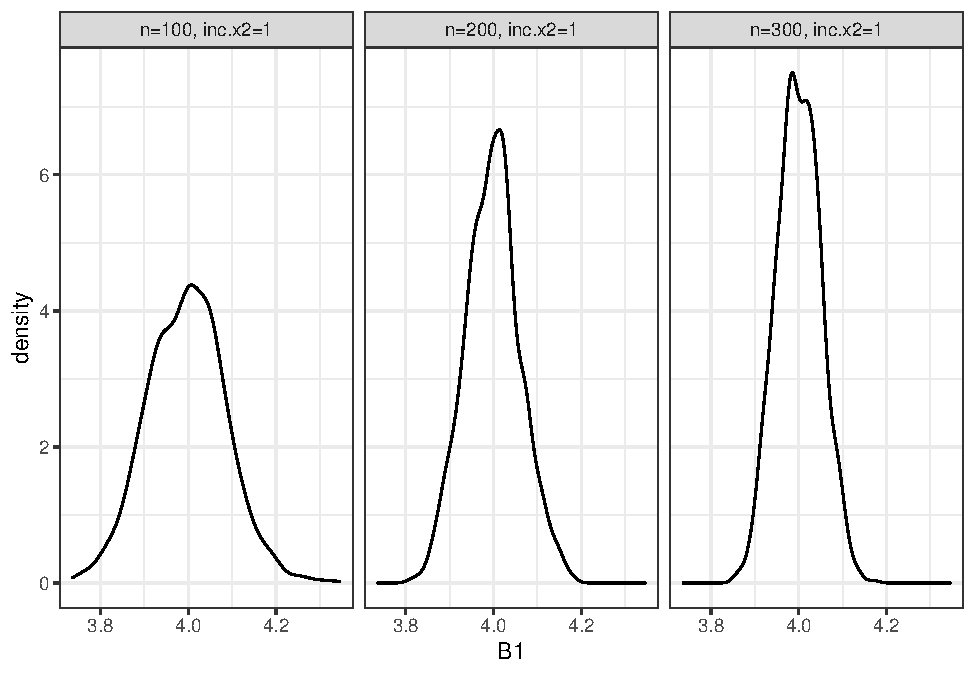
\includegraphics{Report_files/figure-latex/ols_b1-1.pdf}
 \caption{MC \(\beta_1\) results}
 \end{figure}

 \begin{figure}
 \centering
 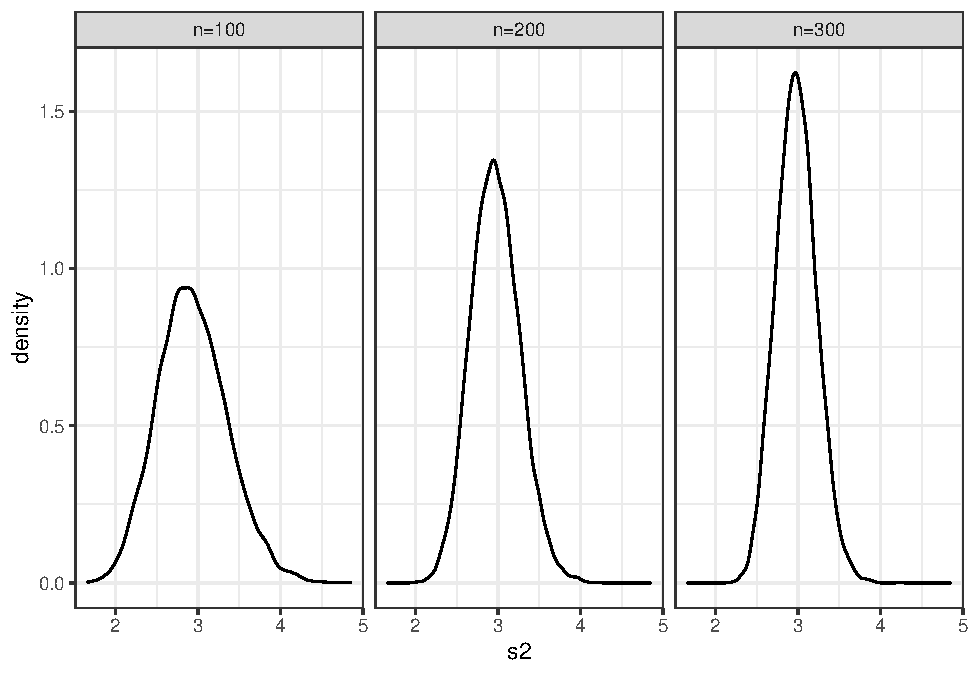
\includegraphics{Report_files/figure-latex/ols_s2-1.pdf}
 \caption{MC \(s^2\) results}
 \end{figure}

 \#\#Ommited variable bias and irrelevant regressor inclusion

 Moreover, another common problem for estimation is the inclusion of
 suitable regressors into the model. Both the inclusion of irrelevant
 variables and the absence of relevant ones into the regression model
 cause problems when estimating the true parameters. In this section, we
 will test the impact both of these problems on the estimated values.
 \noindent We continue with the same structure as in equation
 \eqref{eq_DGP}, we will test, however, the case when \(\beta_2 = 0\)
 which means that \(x_2\) has no influence on \(y\). This causes a
 problem in the estimation when the researcher does not know the
 underlying DGP and includes \(x_2\) to the model, because of lack of
 information or convenience. \textit{A priori} the expected result is
 that the estimated coefficient associated with this new variable will
 be 0, while the variance of the residuals however will increase.

 \noindent We test this hypothesis using a Monte Carlo study, where we
 use the same coefficient values as for the base example, except that we
 set \(\beta_2=0\). Then we run an OLS model with \(x_1\) and \(x_2\) as
 the regressors using \(n = (100, 200, 300)\). Lastly, we repeat this
 10000 times for every value of \(n\). We present the obtained results
 in table \ref{eq:irr_ols_table}. Two panels are presented again, one
 for the mean results of the ten first MC repetitions and the second for
 all repetitions. Again the hypothesis about the behavior of the
 coefficients is proven to be right, i.e.~the estimators for \(\beta_0\)
 and \(\beta_1\) appear to converge to the true value. In contrast, the
 estimator for \(\beta_2\) is marginally different from zero for all
 values of \(n\), and from the overall mean results we conclude that
 this behavior does not change. Lastly, the last point of the hypothesis
 about the estimator of the variance of the error term is also proven to
 be right. This is because the results for the estimator \(s^2\) have
 higher values compared to the ones obtained in table \ref{ols_table}.

 \begin{table}[H]

 \caption{\label{tab:irr_ols_table}MC OLS results with an irrelevant variable}
 \centering
 \begin{tabular}[t]{ccccc}
 \toprule
 Number of observations & $\beta_0$ & $\beta_1$ & $\beta_2$ & $s^2$\\
 \midrule
 \addlinespace[0.3em]
 \multicolumn{5}{l}{\textbf{N = 10}}\\
 \hspace{1em}100 & 0.994 & 4.033 & 0.001 & 2.911\\
 \hspace{1em}200 & 0.951 & 4.007 & 0.009 & 2.860\\
 \hspace{1em}300 & 0.988 & 3.984 & -0.005 & 2.988\\
 \addlinespace[0.3em]
 \multicolumn{5}{l}{\textbf{N = 10000}}\\
 \hspace{1em}100 & 0.998 & 4.000 & 0.000 & 2.935\\
 \hspace{1em}200 & 1.000 & 4.000 & 0.000 & 2.970\\
 \hspace{1em}300 & 1.002 & 4.000 & 0.000 & 2.981\\
 \bottomrule
 \multicolumn{5}{l}{\rule{0pt}{1em}\textit{Note: }}\\
 \multicolumn{5}{l}{\rule{0pt}{1em}Total repetitions = 10000, total parameter combinations = 3}\\
 \end{tabular}
 \end{table}

 Lastly, we test the effects of estimating a model using only \(x_1\)
 when the underlying DGP follows the structure of \eqref{eq_DGP}, this
 problem is most commonly known as having an omitted variable bias. The
 theoretical consequences of this problem are related to the consistency
 and unbiasedness of the estimators. Since it is necessary that \(x_1\)
 and \(x_2\) share a degree of correlation between them, the absence of
 one of them in the regression model will cause the available variable
 to be correlated with the error term, thus violating one of the main
 assumptions of this methodology. This correlation will lead to an
 estimator of \(\beta_1\) to have a higher or lower expected value
 (depending on the sign of the correlation) in comparison to the true
 parameter.

 \hypertarget{package-principles-mcs}{%
 \section{Package Principles \{MCS\}}\label{package-principles-mcs}}

 \hypertarget{vignettevignette}{%
 \section{Vignette\{vignette\}}\label{vignettevignette}}

 Operationally, we test this theoretical behavior using the same
 structure as for the last examples, now however we do not include
 \(x_2\) into our estimated model. We present the results in table
 \ref{tab:ommiols}. To see a clearer difference we present the results
 for both models where \(x_2\) is included and where is not. We see a
 clear difference in the estimated coefficients, on one hand the
 estimated intercept is completely overestimated, averaging around a
 value of 16 no matter the number of observations used or the number of
 MC replications. On the other hand, the estimated variance of the error
 term is also completely overestimated and does not seem to converge to
 the real value. We conclude that the absence of one important variable
 in the model has a bigger impact when compared to the inclusion of an
 irrelevant variable.

 \begin{table}[H]

 \caption{\label{tab:ommiols}Ommited variable bias MC results}
 \centering
 \begin{tabular}[t]{cccccc}
 \toprule
 Number of observations & $x_2$ included or not & $\beta_0$ & $\beta_1$ & $\beta_2$ & $s^2$\\
 \midrule
 \addlinespace[0.3em]
 \multicolumn{6}{l}{\textbf{N = 10}}\\
 \hspace{1em}100 & 0 & 15.702 & 3.427 & NA & 378.464\\
 \hspace{1em}100 & 1 & 0.960 & 4.025 & 5.005 & 2.908\\
 \hspace{1em}200 & 0 & 16.625 & 3.925 & NA & 413.417\\
 \hspace{1em}200 & 1 & 0.967 & 3.983 & 5.008 & 2.827\\
 \hspace{1em}300 & 0 & 16.704 & 3.887 & NA & 408.881\\
 \hspace{1em}300 & 1 & 0.953 & 4.010 & 5.001 & 3.035\\
 \addlinespace[0.3em]
 \multicolumn{6}{l}{\textbf{N = 10000}}\\
 \hspace{1em}100 & 0 & 16.008 & 3.990 & NA & 399.183\\
 \hspace{1em}100 & 1 & 1.000 & 4.001 & 5.000 & 2.941\\
 \hspace{1em}200 & 0 & 15.996 & 4.008 & NA & 400.842\\
 \hspace{1em}200 & 1 & 0.999 & 4.000 & 5.000 & 2.968\\
 \hspace{1em}300 & 0 & 15.985 & 4.001 & NA & 401.614\\
 \hspace{1em}300 & 1 & 1.000 & 4.000 & 5.000 & 2.981\\
 \bottomrule
 \multicolumn{6}{l}{\rule{0pt}{1em}\textit{Note: }}\\
 \multicolumn{6}{l}{\rule{0pt}{1em}Total repetitions = 10000, total parameter combinations = 6}\\
 \end{tabular}
 \end{table}

 \hypertarget{comparison-to-other-monte-carlo-approaches-in-rcomparsion}{%
 \section{Comparison to other Monte Carlo Approaches in
 R\{comparsion\}}\label{comparison-to-other-monte-carlo-approaches-in-rcomparsion}}

 \hypertarget{conclusion}{%
 \section{Conclusion}\label{conclusion}}

 With the tidyMC package we provide research an easy and confortable way
 to to Monte Carlo Studies.

 \hypertarget{strucutre}{%
 \section{Strucutre}\label{strucutre}}

 -Introduction to MCS (5) - How it works in our package (10) -
 parallelisation plan - function - return objects - objects - summary -
 plots - tables - exampl of outputs - extension: bootstrap - Comparison
 to Monte Carlos package (3) - objects - speed -bench::mark - Vignette

 \textbackslash end\{document\}
			\renewcommand*{\mkbibnamefamily}[1]{\textbf{#1}}
	\renewcommand*{\mkbibnamegiven}[1]{\textbf{#1}}
	\renewcommand*{\mkbibnameprefix}[1]{\textbf{#1}}
	\renewcommand*{\mkbibnamesuffix}[1]{\textbf{#1}}
	\printbibliography[title=References]
		\end{document}